\section{数据库设计}

\subsection{ER 图}

\begin{figure}[H]
\centering
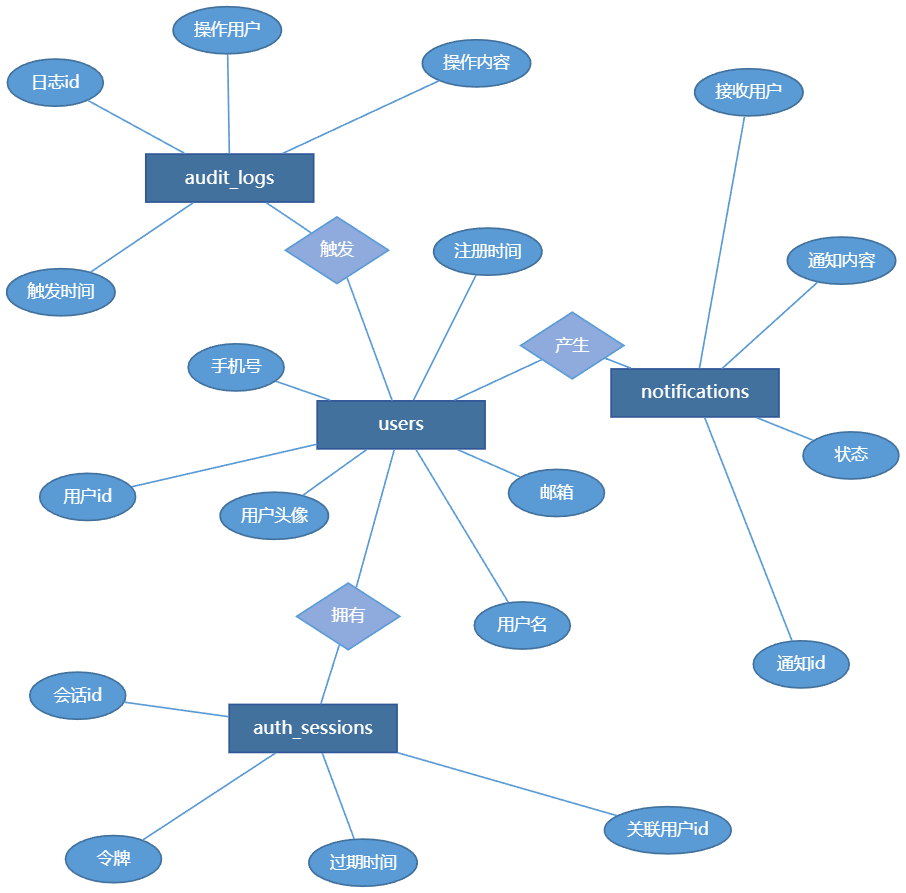
\includegraphics[height=0.45\textheight]{figures/er1.png}
\caption{用户与安全鉴权模块 ER 图}
\label{fig:er-auth}
\end{figure}

\begin{figure}[H]
\centering
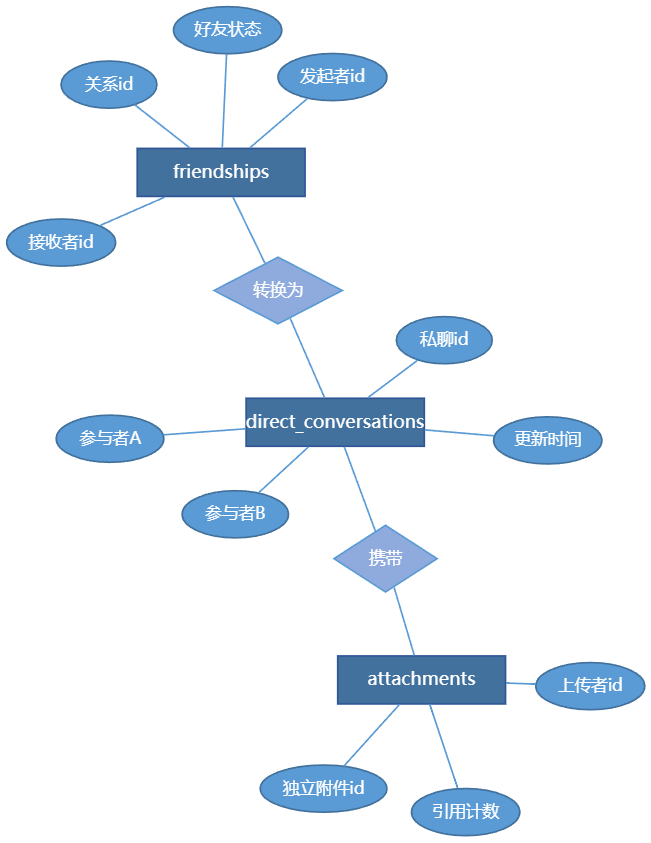
\includegraphics[height=0.40\textheight]{figures/er2.png}
\caption{社交关系与私聊模块 ER 图}
\label{fig:er-social}
\end{figure}

\begin{figure}[H]
\centering
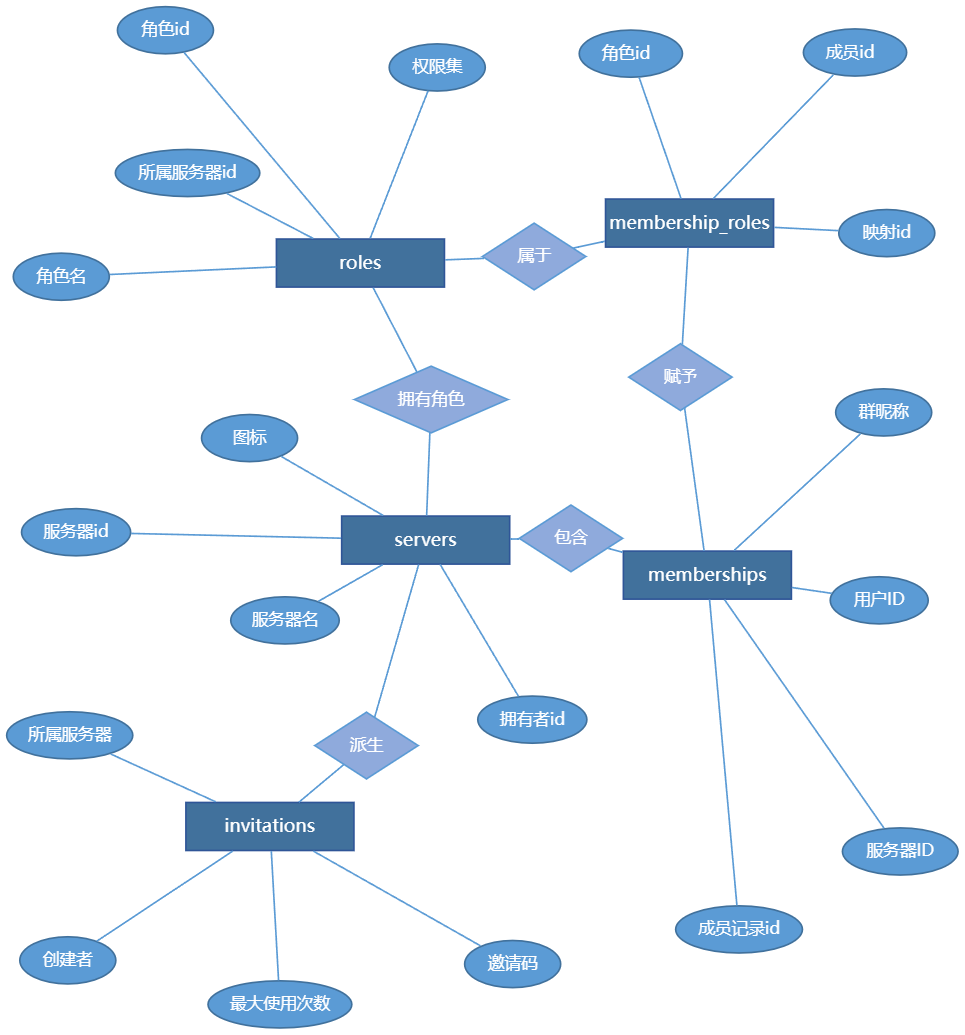
\includegraphics[height=0.45\textheight]{figures/er3.png}
\caption{服务器与成员权限模块 ER 图}
\label{fig:er-server}
\end{figure}

\begin{figure}[H]
\centering
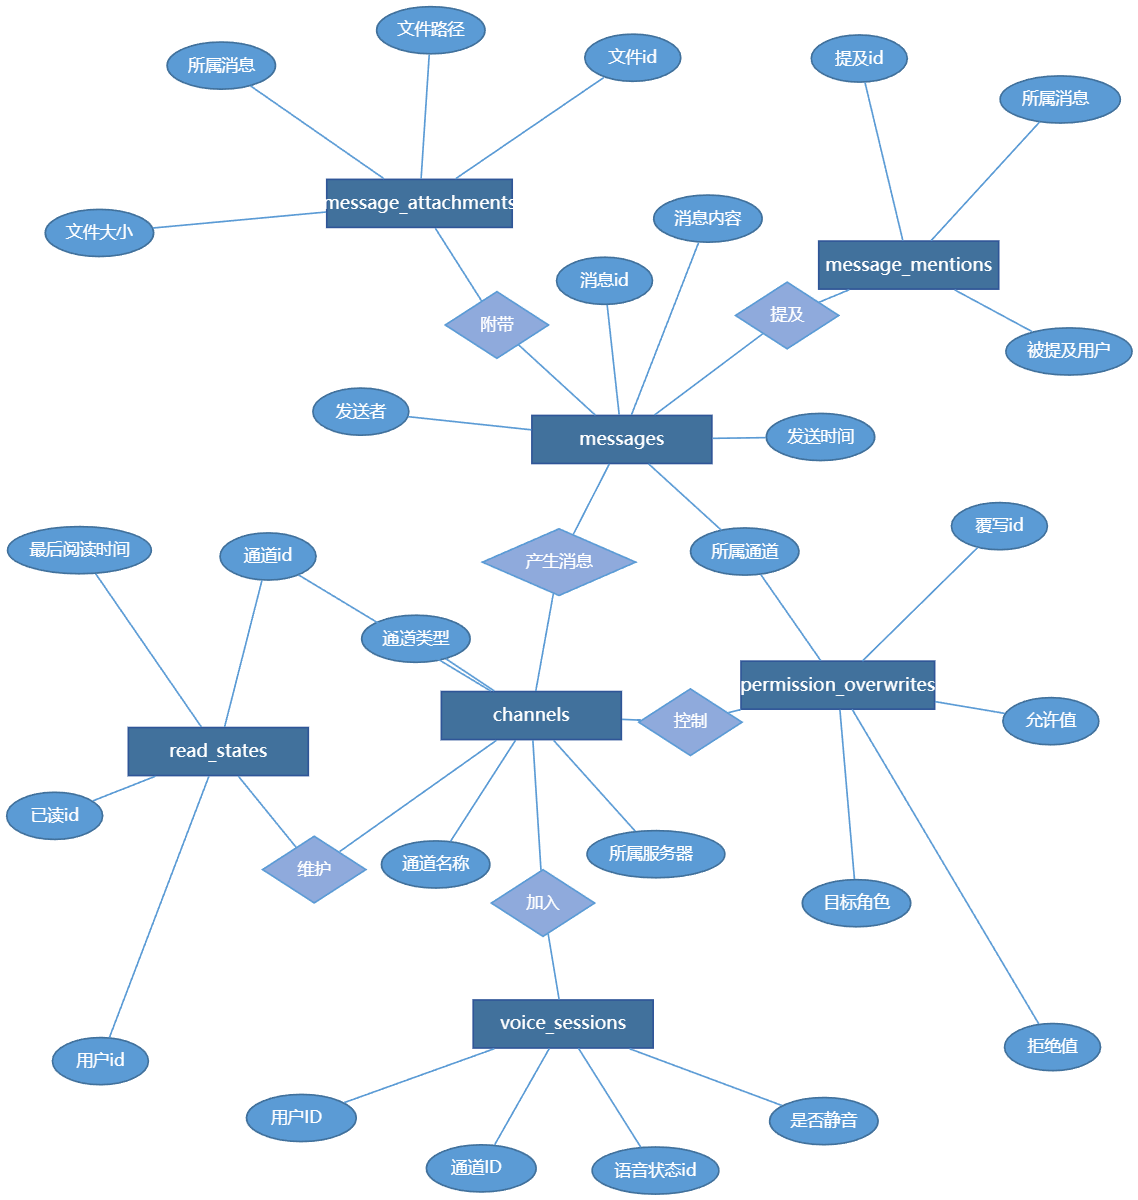
\includegraphics[height=0.50\textheight]{figures/er4.png}
\caption{频道、消息与状态模块 ER 图}
\label{fig:er-channel}
\end{figure}

\subsection{表设计}

系统共 19 个数据模型，以下按业务域分组说明核心实体的关键字段。

\subsubsection{用户与认证}

\noindent\begin{tabularx}{\textwidth}{L{3.2cm}Y}
\toprule
\textbf{表名} & \textbf{关键字段} \\
\midrule
users & id(PK), username(UQ), email\_or\_phone(UQ), password\_hash, nickname, account\_status, presence\_status \\
auth\_sessions & id(PK), user\_id(FK), refresh\_token\_hash(UQ), expires\_at, revoked\_at \\
attachments & id(PK), owner\_id(FK), storage\_key, file\_name, mime\_type, size\_bytes, purpose, status \\
\bottomrule
\end{tabularx}

\subsubsection{社交与好友}

\noindent\begin{tabularx}{\textwidth}{L{3.2cm}Y}
\toprule
\textbf{表名} & \textbf{关键字段} \\
\midrule
friendships & id(PK), requester\_id(FK), addressee\_id(FK), status(pending/accepted/rejected/deleted) \\
direct\_conversations & id(PK), participant\_a\_id(FK), participant\_b\_id(FK), last\_message\_id(FK) \\
notifications & id(PK), user\_id(FK), type, source\_type, source\_id, dedupe\_key(UQ), is\_read \\
\bottomrule
\end{tabularx}

\subsubsection{社区与权限}

\noindent\begin{tabularx}{\textwidth}{L{3.2cm}Y}
\toprule
\textbf{表名} & \textbf{关键字段} \\
\midrule
servers & id(PK), owner\_id(FK), name, icon\_attachment\_id, description, status \\
invitations & id(PK), server\_id(FK), code(UQ), created\_by\_id(FK), expires\_at, max\_uses, used\_count \\
memberships & id(PK), server\_id(FK), user\_id(FK), nick\_in\_server, member\_status \\
roles & id(PK), server\_id(FK), name, permission\_bits(BigInt), color, priority, is\_default \\
membership\_roles & membership\_id(FK), role\_id(FK)（联合主键）\\
permission\_overwrites & id(PK), channel\_id(FK), target\_type, target\_id, allow\_bits, deny\_bits \\
\bottomrule
\end{tabularx}

\subsubsection{频道、消息与语音}

\noindent\begin{tabularx}{\textwidth}{L{3.2cm}Y}
\toprule
\textbf{表名} & \textbf{关键字段} \\
\midrule
channels & id(PK), server\_id(FK), name, type(TEXT$|$VOICE), sort\_order \\
messages & id(PK), scope\_type, channel\_id, conversation\_id, sender\_id(FK), content, visibility, client\_message\_id \\
message\_attachments & message\_id(FK), attachment\_id(FK)（联合 PK）\\
message\_mentions & message\_id(FK), mentioned\_user\_id(FK)（联合 PK）\\
read\_states & id(PK), user\_id(FK), scope\_type, channel\_id, conversation\_id, last\_read\_message\_id, unread\_count \\
voice\_sessions & id(PK), channel\_id(FK), user\_id(FK), mute\_state, deafen\_state, connection\_status, router\_id, producer\_id \\
audit\_logs & id(PK), actor\_id(FK), action, result, target\_type, target\_id, metadata(JSONB) \\
\bottomrule
\end{tabularx}